\section{יישום המודל בממשק דיגיטלי תומך החלטה}
כחלק מהמעבר ממודל מחקרי לכלי יישומי, פותח ממשק דיגיטלי המאפשר להריץ את שרשרת החיזוי ללא צורך בכתיבת קוד. מטרת הממשק היא להנגיש את מודל החיזוי למשתמש תפעולי, ולאפשר קבלת תחזית עתידית של ערכי pH ו-EC בבית השורשים על בסיס נתוני אקלים, קרינה, השקיה, דישון ומדידה נוכחית ידועה.

הממשק משמש כשכבת הפעלה מעל המודלים שפותחו בפרויקט: תחילה מופעל מודל המיקרו-אקלים, אשר יוצר תחזית של תנאי הסביבה בתוך החממה, ולאחר מכן מופעל מודל בית השורשים, המשתמש בתחזית זו יחד עם נתוני הממשק החקלאי כדי לחזות את מצב ה-pH וה-EC בנקודת זמן עתידית.

\subsection{מטרת הממשק}
הממשק נועד לגשר בין שלב הפיתוח המחקרי לבין שימוש מעשי במודל. בעוד שבשלב המחקר המודלים הופעלו באמצעות מחברות Jupyter וקוד Python, הממשק מאפשר למשתמש להזין נתונים בצורה מובנית, להריץ את המודלים ולקבל פלט ברור של תחזית בית השורשים.

באופן זה, המערכת הופכת את מודל ה־\SoftSensor{} לכלי תומך החלטה ראשוני. המשתמש אינו נדרש להבין את פרטי המימוש של המודל, אלא רק לספק את הקלטים הדרושים: נתוני מזג אוויר וקרינה, ערכי pH ו-EC נוכחיים, מועד החיזוי, ונתוני אירועי השקיה ודישון רלוונטיים.

\subsection{מבנה תהליך העבודה בממשק}
תהליך העבודה בממשק מחולק לארבעה שלבים מרכזיים:

\begin{enumerate}
    \item \textbf{העלאת נתוני אקלים וקרינה:} בשלב הראשון המשתמש מעלה קובצי מזג אוויר וקרינה. המערכת תומכת בקבצים בפורמטים נפוצים כגון CSV, Excel ו-JSON. נתונים אלו משמשים כקלט למודל המיקרו-אקלים.
    \item \textbf{יצירת תחזית מיקרו-אקלים:} לאחר העלאת הקבצים, המערכת מפעילה את מודל המיקרו-אקלים ומייצרת תחזית של משתנים פנימיים בחממה, כגון טמפרטורה, לחות, ET0, קרינה פנימית וטמפרטורת קרקע. תחזית זו נשמרת כקובץ פלט, ומשמשת בהמשך כקלט למודל בית השורשים.
    \item \textbf{הזנת מצב בית השורשים ואירועים תפעוליים:} בשלב זה המשתמש מזין את נקודת הבסיס של החיזוי: זמן המדידה הנוכחית, ערכי pH ו-EC נוכחיים, זמן היעד לחיזוי, תאריך שתילה וכיסוי נוף. בנוסף, ניתן להזין אירועי השקיה, דישון, חומצה, Gypsum ו-Kortin שהתרחשו לפני ואחרי נקודת הבסיס. אירועים אלו מספקים למודל את ההקשר התפעולי הנדרש להבנת מצב המצע.
    \item \textbf{הרצת מודל בית השורשים וקבלת תחזית:} לאחר הזנת כל הקלטים, המערכת מפעילה את מודל בית השורשים ומחזירה תחזית לערכי pH ו-EC בנקודת הזמן העתידית. בנוסף, הממשק מציג את פער הזמן בין נקודת הבסיס לנקודת היעד, ומאפשר הורדת קובצי הפלט לצורך תיעוד או ניתוח נוסף.
\end{enumerate}

\begin{figure}[H]
    \centering
    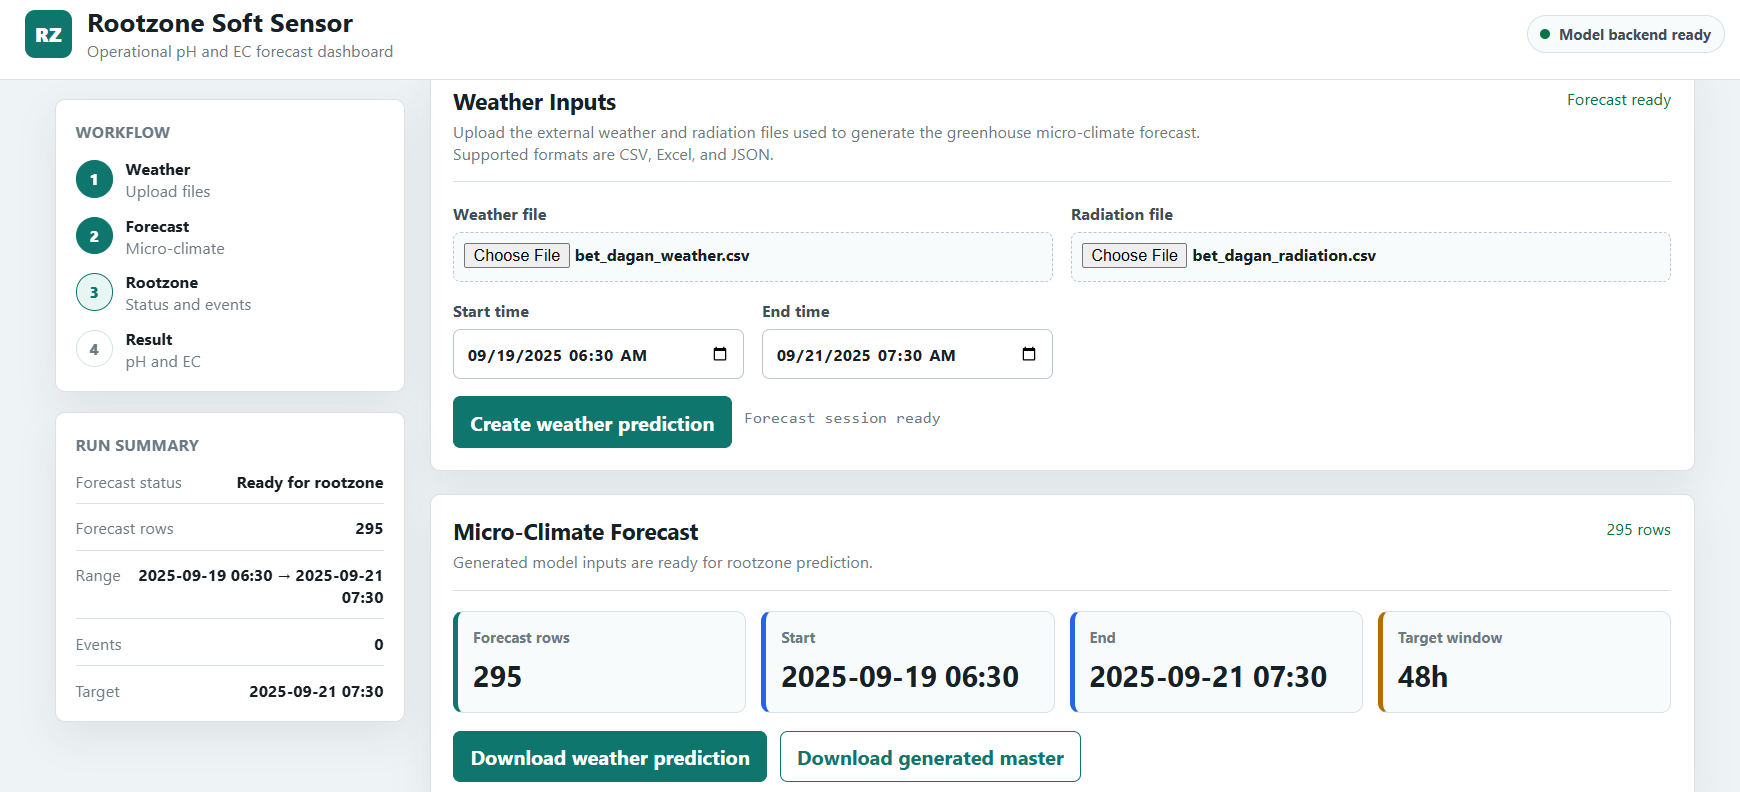
\includegraphics[width=0.95\textwidth]{figures/fig13.png}
    \caption{\LR{Digital Interface -- Weather Upload and Climate Forecast}}
    \label{fig:interface1}
\end{figure}

\begin{figure}[H]
    \centering
    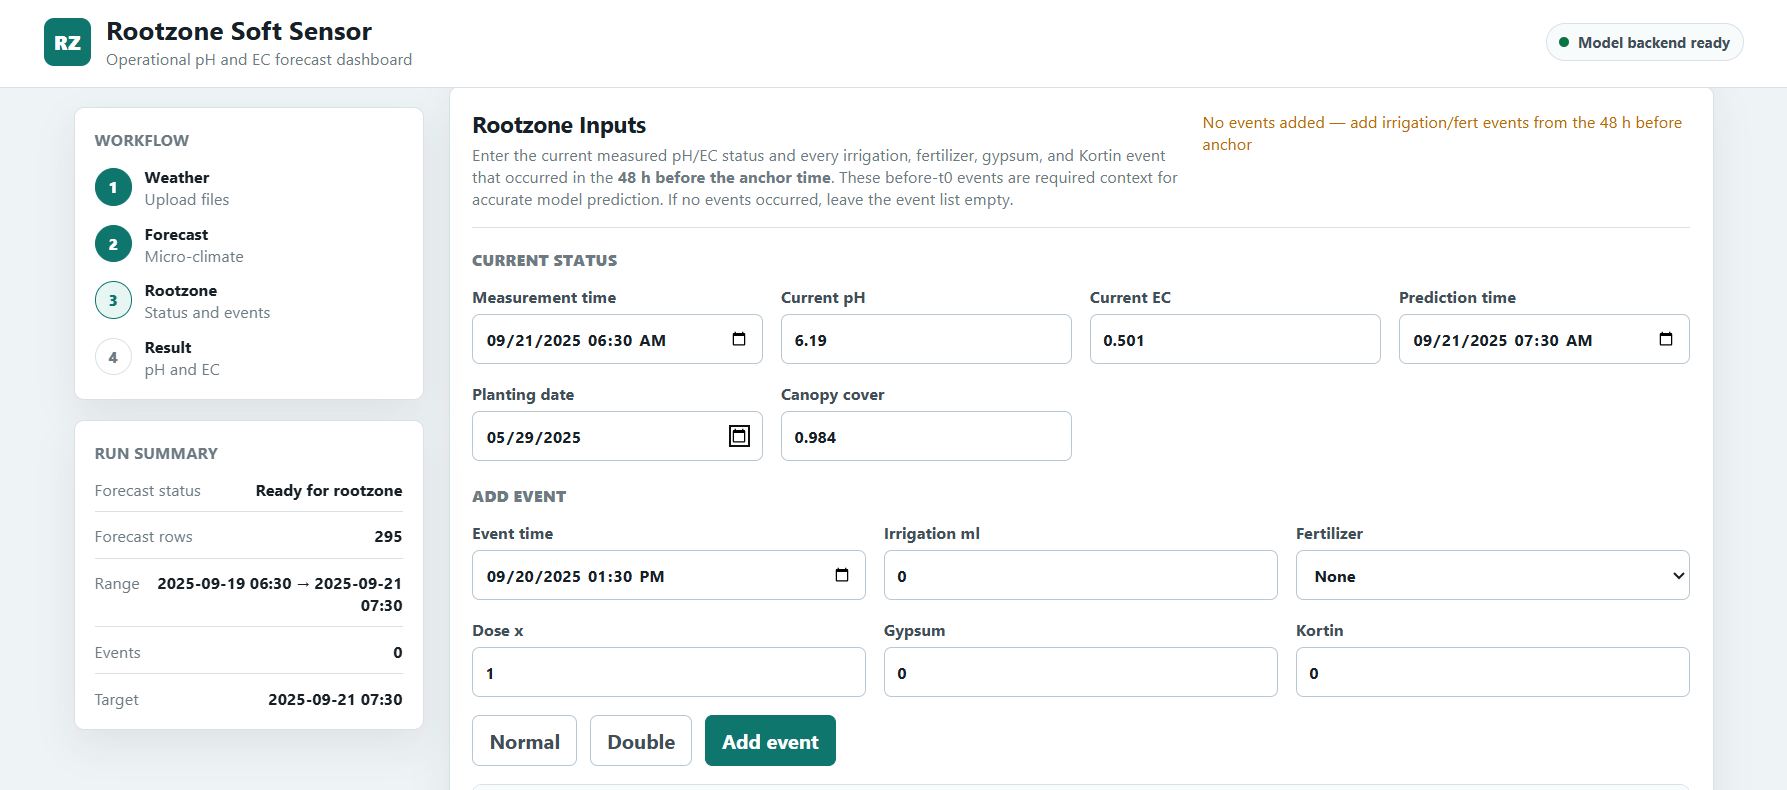
\includegraphics[width=0.95\textwidth]{figures/fig14.png}
    \caption{\LR{Digital Interface -- Operational Inputs}}
    \label{fig:interface2}
\end{figure}

\begin{figure}[H]
    \centering
    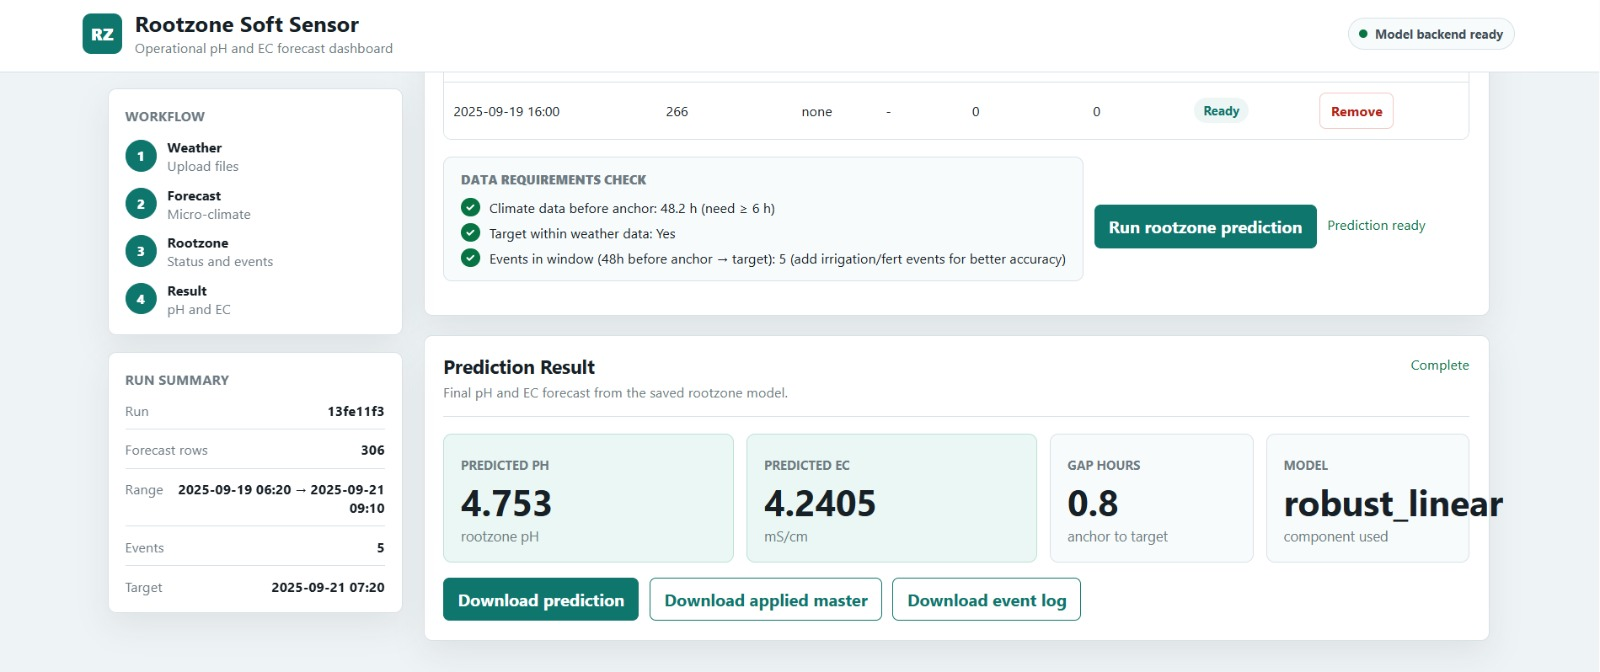
\includegraphics[width=0.95\textwidth]{figures/fig15.jpeg}
    \caption{\LR{Digital Interface -- Rootzone pH and EC Forecast}}
    \label{fig:interface3}
\end{figure}

\subsection{קלטי ופלטי המערכת}
הממשק מקבל מספר קבוצות קלט מרכזיות. תחילה מוזנים קובצי מזג אוויר וקרינה, המשמשים ליצירת תחזית מיקרו-אקלים בתוך החממה. לאחר מכן מוזנים ערכי pH ו-EC נוכחיים, זמן המדידה, זמן היעד לחיזוי, נתוני מצב הצמח, ואירועי השקיה ודישון שהתרחשו בפרק הזמן הרלוונטי.

שילוב קלטים אלו מאפשר למודל להתייחס לא רק למצב הנוכחי של בית השורשים, אלא גם לתנאים הסביבתיים ולפעולות הממשק שהתרחשו בין נקודת הבסיס לנקודת החיזוי. בכך הממשק משמר את מבנה החיזוי של המודל, המבוסס על מעבר מ-$t_0$ ל-$t_1$ ולא על חיזוי רגעי מנותק מהקשר.

פלטי המערכת כוללים את ערך ה-pH החזוי, ערך ה-EC החזוי ביחידות mS/cm, מספר השעות בין נקודת הבסיס לנקודת היעד, וקובצי פלט להורדה. קבצים אלו כוללים את תחזית המיקרו-אקלים, טבלת הנתונים המעובדת ותחזית בית השורשים, ויכולים לשמש לתיעוד, בדיקה או ניתוח נוסף.

\subsection{חשיבות הממשק בפרויקט}
הממשק הדיגיטלי מהווה שלב חשוב בהפיכת המודל מכלי מחקרי לכלי תומך החלטה יישומי. הוא מאפשר להפעיל את שרשרת החיזוי בצורה מובנית, להפחית תלות בקוד, ולבדוק כיצד המודל עשוי להשתלב בתהליך עבודה חקלאי.

עם זאת, בשלב הנוכחי הממשק אינו מהווה מערכת בקרה אוטונומית ואינו מחליף שיקול דעת מקצועי או מדידות ידניות. תפקידו הוא לספק הערכה עתידית של מצב בית השורשים, שתוכל לסייע למגדל או לאגרונום לזהות מגמות אפשריות ולקבל החלטות מושכלות יותר לגבי השקיה, דישון או צורך במדידה נוספת.
